\section{Introduction}

The Job Provenance (\JP) service is primarily designed to provide a permanent
storage and advanced querying interface to the data about Grid jobs and
the environment they were run in. This information is to be used for
statistical purposes, lookup for patterns in the Grid behavior and also
for job re-submission.

The Job Provenance extends the data model specified by the \LB service 
with additional information about each job---most specifically the input
and output data files---and also information about the run time
environment. 

The Job Provenance must fulfill rather contradictory requirements. It
must keep detailed information about each job, the environment the job
run in and the affected files, as possible. On the other hand, being a
permanent service, the job records must be kept reasonably small
to fit into reasonable sized storage system. Given the expected number of
jobs on large scale Grids---\eg the EGEE already
reports\footnote{\url{http://egee-jra2.web.cern.ch/EGEE-JRA2/QoS/JobsMetrics/JobMetrics.htm}}
20k jobs per day, that is 7.5M jobs per year, a number of jobs before the
large experiments will be deployed---the \JP must also support very
efficient searching and querying features. Another problem is associated
with the long life span of the \JP service. It must be expected that the
data formats will change over the time, while the \JP is expected to deal
with old and new data formats in a uniform way. They can be achieved via 
extensibility of the JP data model.

As the data collection serviced by the JP will extensively grow, it is
impossible to rely only on the primary data when navigating through it.
Users must be able to add annotations to individual job records and these
annotations serve two primary purposes---to help in organizing the \JP
data and to be a source of additional information, not provided directly
by the automated collection of primary data. Even annotations must follow
the WORM (write once read many times) semantics, as they are always added
on top of the already stored data, never re-writing the old annotations.
Work with the most recent set of annotations as well as ability to
inspect the history of annotations must be supported.

Fig.~\ref{fig:psinter} depicts interaction between Job Provenance and
other Grid middleware components (on the example of the gLite
infrastructure).
\begin{figure}[ht]
  \centering
  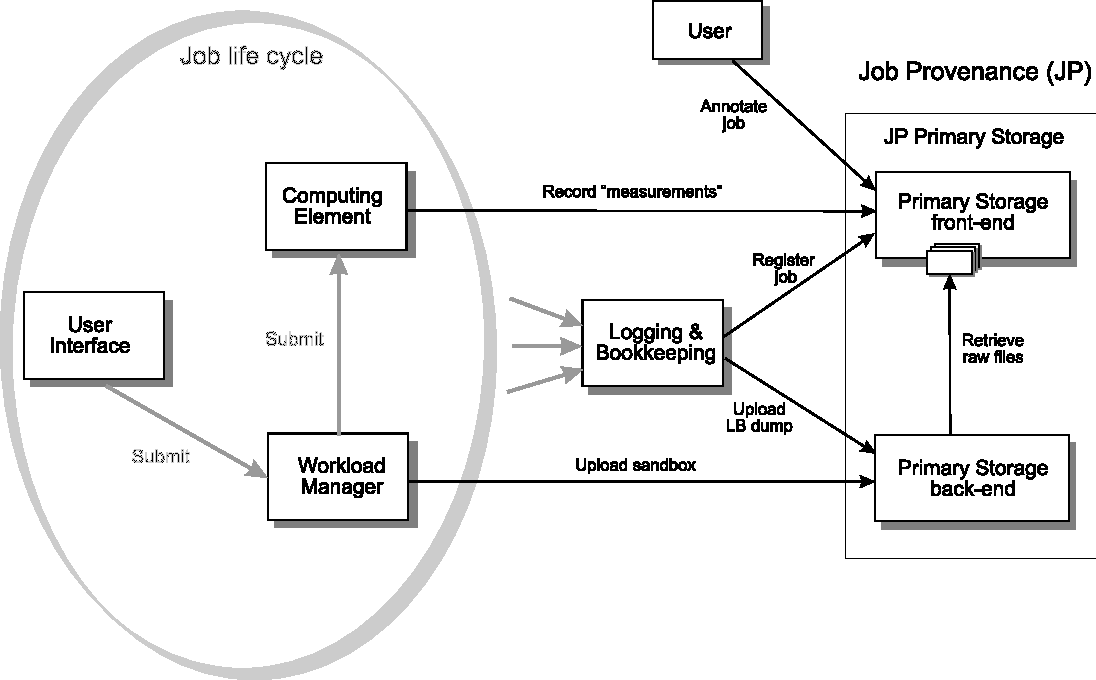
\includegraphics[scale=0.5]{images/JP-interactions}
  \caption{Data flow into gLite Job Provenance}
  \label{fig:psinter}
\end{figure}

\subsection{Concepts}
\ludek{\TODO{Obrazky moc nezapadaji do soucasne struktury textu :-(}}

\subsubsection{Data gathering}%
\label{data}
%\begin{comment}
%\todo{job record, job attributes} \todo{open design, scalable}
%\todo{we have very small persistent record (jobid, owner, timescale),
%  set of associated files and we maintain corresponding plugins (by what?) to
%  interpret them; metadata are mined, indexed and provided on demand}
%\todo{attribute namespaces---a glue to source of metadata}
%\end{comment}

The primary data organization in \JP is on a per job basis, a concept
taken from the \LB data organization. Every data item stored in JP is
associated to a~particular Grid job. As the overall storage capacity
requirements may become enormous, we store only volatile data which are
neither stored reliably elsewhere nor are reproducible by the job.
The data gathered from the gLite middleware fall into the following categories:
\begin{itemize}
\item job inputs, directly required for job re-running
\begin{itemize}
\item complete job description (JDL) as submitted to WMS
\item miscellaneous input files (gLite WMS input sandbox) provided by the user
(but job input files from remote storage \emph{are not} copied to JP)
\end{itemize}
\item job execution track, witnessing the environment of job execution
\begin{itemize}
\item complete \LB data, for example when and where the job was
  planned and executed, how many times and for what reasons it was
  resubmitted etc.
\item ``measurements'' on computing elements, \eg versions of installed
software, environment settings etc.
\end{itemize}
\end{itemize}
In addition, the service allows the user to add arbitrary annotations to
a~job in a form of ``name = value'' pairs.
These annotations can be recorded either during the job execution or at any time
afterward.
Besides providing information on the job (\eg it was a~production-phase
job of a particular experiment) these annotations may carry 
information on relationships between the job and other entities
like external datasets, forming the desired data provenance record.

%\TODO{zduraznit WORM semantiku + citace na IPAW}
Once a~piece of data is recorded for a~job, it can be never updated or
replaced.
New values can be recorded%
\footnote{It seems to make sense only for the annotations, not the
middleware data, and the current implementation makes this restriction.
However, it can be relaxed without principal impact.}
but the old values are always preserved.
Consequently the recorded history cannot be lost.


\subsubsection{Data representation}%
\label{attrib}

The \JP concept distinguishes between two views on the processed data. 
The data are stored in the \JP in the \emph{raw representation}.
Two input modes are assumed, depending mainly on the size
and structure of the data:
\begin{itemize}
\item Small size \emph{tags} in a form of ``name = value'' pairs,
enter the system via its primary interface (as a~web service operation
in the current implementation).
``Value'' is assumed to be a literal, without any structure that \JP should
be aware of.

\item \emph{Bulk files}, \eg the complete dump of \LB data or the job input
sandbox, are uploaded via a~suitable transfer protocol%
\footnote{The current implementation supports \texttt{gsiftp://} only but 
other protocols can be easily added.}.
Files are supposed to be structured.
However, they are stored ``as is'', and upon upload they are annotated with
format identification, including version of the format.
JP allows installing plugins that handle particular file formats (see bellow),
understanding the file structure and extracting required information.
\end{itemize}

Most data manipulation is done using the \emph{logical view}. 
Any piece of information stored in JP is represented
as a~value of a particular named \emph{attribute}. Tags (user
annotations) map to attributes in a~straightforward way, name and value
of the tags becoming name and value of an attribute. An uploaded file is
usually a~source of multiple attributes, which are automatically extracted
via \emph{plugins}. JP defines a~\emph{file-type plugin interface API}. The
task of the plugin is parsing a~particular file type and providing calls
to retrieve attribute values.

To avoid naming conflicts even with future attributes, 
an attribute name always falls into a~namespace.
Currently we declare three different namespaces: for JP system attributes
(\eg job owner or
registration time), attributes inherited from \LB, and unqualified user tags.

\ludek{
This representation unifies the user annotations, the ``system''
middleware data and information extracted from uploaded files into
a~single view.}

\iffalse
An attribute value must be always representable in the form of a~printable
string.
If it is not the case for a~native attribute type, 
converting rules must be provided by a~plugin (dynamically loadable library)
implementing a~specified API.
\fi

We keep the scheme symmetric, which means that none of the currently declared attribute
namespaces is privileged in any sense.
However, it may present a~vulnerability\Dash a~malicious user may try 
to override a~\JP system attribute using the user annotation interface.
Therefore each attribute value carries a~further \emph{origin classification}:
currently \emph{system}, \emph{user} (recorded as tag), and
\emph{file} (found in an uploaded file).

Finally, as JP does not support updating data intentionally
(see Sect~\ref{data}), multiple values of an attribute are allowed.
The order in which the values were recorded can be reconstructed from
timestamps attached to each value, getting the ``attribute update'' semantics
if it is required.

Attributes, representing the logical view, is the only way to specify queries on JP.
However, once the user knows an~actual jobid, bulk files can be retrieved
in the raw form, too (assumed to be useful in the case of input sandboxes
reused for job re-execution).

\subsubsection{Layered architecture}%
\label{layered}
\JP is formed of two classes of services: the permanent \emph{Primary Storage}
(JPPS) accepts and stores job data
while possibly volatile and configurable \emph{Index Servers} (JPIS)
provide an optimized querying and data-mining interface to the end-users.

The expected large amount of stored data yields a requirement on
maximal compactness of the storage.
The raw data should be compressed,
and the set of metadata kept with each job must be minimal.
\JP defines a~set of \emph{primary attributes} which are maintained
by JPPS for each job.
Jobid is the only mandatory primary attribute,
other suggested ones are the job owner, submission time,
and the virtual organization.
All other attributes are retrieved from the raw data only when requested.

The restricted set of primary attributes prohibits user queries to be served
by the JPPS directly (with the only exception of the known jobid).
Due to the expected low selectivity of primary attributes such queries
would result in processing large number of job records, overloading
the server when the queries became frequent.

These contradictory requirements (compactness vs. performance) had to be
resolved at another component layer.
The main idea is preprocessing the huge \JP dataset with several queries,
each of them covering a~superset of one expected class of user queries
(\eg jobs of particular VO, submitted in certain period).
If these super-queries are chosen carefully, they retrieve only a~small
fraction of the primary data. Their results can thus be stored (or cached)
in a~richer form, including various indices, hence being suitable
for fast response to user queries.
Querying JPPS in this way and maintaining the cache of the query result
is the task of Index Servers in the \JP architecture.

Relationship of JPPS and JPIS is a many-to-many---a~single JPIS can query
multiple JPPS's and vice versa, a~single JPPS is ready to feed multiple JPIS's.

The query conditions restrict the dataset in terms of the matching job records.
Similarly, the query specifies a~set of attributes to retrieve,
reducing also considerably the amount of retrieved data per each matching job.

Index Servers query JPPS in two modes: in \emph{batch mode} JPIS is populated
with all JPPS content matching the query. In this way JPIS can be created
from scratch, despite the ope-ration is rather heavy for JPPS.
On the other hand, the \emph{incremental mode} allows JPIS to subscribe with
JPPS to receive new matching records as well as updates to already stored
records whenever new data arrive to JPPS.
This mode allows existing JPIS to be kept up to date while it is 
still lightweight for JPPS.

Finally, the described layer of JPIS's needn't be the only one.
The architecture (despite not the current implementation) allows
building another layer of JPIS's with many-to-many relationship with
the previous layer instances, combining their data, providing support
for other specific user queries etc.

\subsection{Prototype implementation}

The \JP prototype implementation%
\footnote{a part of the gLite middleware 3.x}
follows the described architecture.

\subsubsection{Primary Storage}%
\label{primary}
\iffalse
The JP \emph{Primary Storage} (JPPS) is a~permanent service responsible
for gathering the job data and their long-term archival.
The primary data are kept in as compact form as possible, and
only minimal metadata (jobid and owner, registration time) are maintained
and indexed.
\fi

A~single instance of JPPS, shown in Fig.~\ref{fig:psinter},
is formed by a~front-end, exposing
its operations via a~web-service interface%
\footnote{Described in detail in ``EGEE Middleware
Design'',\\ \url{https://edms.cern.ch/document/487871/},
documented web service definitions can be found at \\
\url{http://egee.cesnet.cz/en/WSDL/}}%
, and a~back-end, responsible
for actual data storage and providing the bulk file transfer interface.
The front-end metadata (the primary attributes for each job,
authorization information, and JPIS subscription data)
are stored in a~relational database (currently MySQL).

The back-end uses Globus \texttt{gridftp} server enriched with authorization
callbacks accessing the same database to check whether a~user
is allowed to upload or retrieve a~given file.
Both the front- and back-ends share a~filesystem so that the file-type plugins
linked into the front-end access their files via POSIX~I/O.

JPPS operations fall into the following categories:
\begin{itemize}
\item\emph{Job registration.}
Each job has to be explicitly registered with JP.
Currently the registration is done transparently by the \LB server
upon job submission (in parallel with the job registration in \LB,
though not blocking the job submission).

\item\emph{Tag recording.}
Add user tags (annotations) in the ``name = value'' form to JP job records.

\item\emph{Bulk file upload.}
File properties (type, optional name etc.)
are specified via the front-end interface, the upload itself goes
directly to the back-end (using \texttt{gridftp} transfer).

\item\emph{Index Server feed} allows JPIS to ask for batch feed 
as well as register for incremental updates.

\item\emph{Data retrieval.}
The only direct data retrieval supported by JPPS is keyed by
the jobid. 
Both individual attributes and the whole files can be retrieved.
\end{itemize}

Primary Storage covers the first set of requirements specified
for a Job Provenance (see Sect.~\ref{jp:req}), \ie storing a~compact job
record, allowing the user to add annotations, and providing elementary
access to the data.

\subsubsection{Index Server}
Index Servers are created, configured, and populated  semi-dynamically
according to particular user community needs. 
The configuration is formed by:
\begin{itemize}
\item one or more Primary Storages to contact,
\item conditions (expressed in terms of \JP attributes) 
on jobs that should be retrieved,
\item list of attributes to be retrieved,
\item list of attributes to be indexed\Dash a~user query must refer
to at least one of these for performance reasons.
\end{itemize}
The set of attributes and the conditions specify the set of data that
is retrieved from JPPS, and they reflect the assumed pattern
of user queries.

The current JPIS implementation keeps the data also in a~MySQL database.
Its schema is flexible, reflecting the server configuration
(columns are created to hold particular attribute value, as well as indices).

The JPIS interface operations fall into the following categories:
\begin{itemize}
\item\emph{Responses to user queries.} 
A~query specifies a~set of attributes to retrieve and
conditions determining the set of matching jobs.
The structure of the query language is identical to~\LB---%
it allows two-level nesting of comparisons of an attribute
with a~constant value.

\item\emph{JPIS-JPPS communication} implements the data flow from JPPS to JPIS.

\item\emph{Administrative} calls to change JPIS configuration
without interfering with its normal operation.
\end{itemize}


\iffalse	% puvodni text, pouzity jen jako zdroj materialu v predchozim

The role of \emph{Index Servers} (JPIS) is processing and re-arranging the data
from Primary Storage(s) into a~form suitable for frequent and complex user
queries.

We can divide implemented operation into three categories:
\begin{description}
\item[Responses to user queries.] 
The main purpose of JPIS is to enable user complex queries.

\begin{itemize}
\item The \texttt{QueryJobs} operation enables to ask the user query and
specify which attributes of matched jobs are returned.
\end{itemize}

\item[JPIS-JPPS communication.] Internal call enabling data exchange between.
JPIS and JPPS.
\begin{itemize}
\item The \texttt{UpdateJobs} Called by JPPS as a response to \texttt{FeedIndex}
request. Updates information on jobs in JPIS, according to what JPPS
currently knows.
\end{itemize}

\item[Administration.] Admin calls for changing configuration on the fly.
\begin{itemize}
\item The \texttt{AddFeed} Called by JPIS admin tool to ask new  primary storage server to feed it. Updates information on JPPS in index server, according to what JPPS currently knows.
\item The \texttt{GetFeedIDs} Called by JPIS admin tool to find out its open feeds. 
\item The \texttt{DeleteFeed} Called by JPIS admin tool to remove one feed session.
\end{itemize} 

\end{description}


\subsubsection{Index Server} 
\label{index}
%\begin{wrapfigure}{r}{.5\hsize}
\begin{figure}
  \centering
  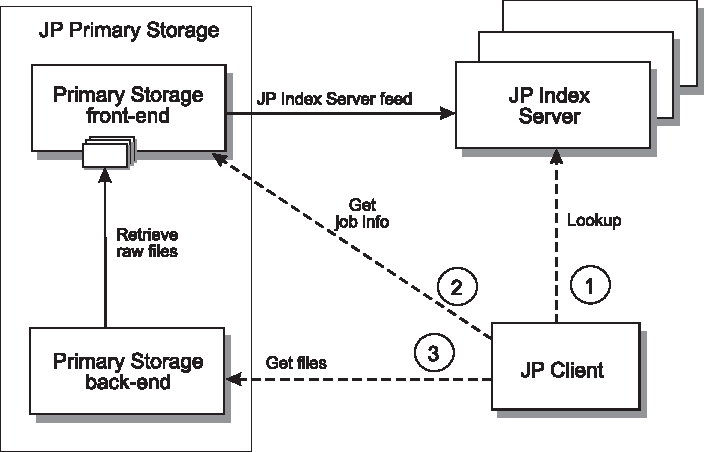
\includegraphics[scale=0.5]{images/JP-query}
  \caption{Index Server interactions}
  \label{fig:query}
\end{figure}
%\end{wrapfigure}



A~typical  interaction is shown in Fig.~\ref{fig:query}.%\\[-8mm]

\begin{enumerate}
\item The user queries one or more JPIS, receiving a~list of ID's
of matching jobs.
\item JPPS is directly queried for additional job attributes or URL's of 
stored files.
\item The required files are retrieved.
\end{enumerate}

The current format of the user query is a~list of lists of conditions.
A~condition is comparison (less, greater, equal) of an attribute 
\wrt\ a~constant. Items of an~inner list must refer to the same attribute
and they are logically or-ed.
Finally the inner lists are logically and-ed. 
According to our experience with the \LB\ service,
this query language is powerful enough to satisfy user needs 
while simple enough to allow efficient implementation.

Index Servers are created, configured, and populated  semi-dynamically
according to particular user community needs. 
The configuration is formed by:
\begin{itemize}
\item one or more Primary Storages to contact,
\item conditions on jobs that should be retrieved,
\item list of attributes to be retrieved,
\item list of attributes to be indexed\Dash a~user query must refer
to at least one of these for performance reasons.
\end{itemize}
The set of attributes and the conditions specify the set of data that
is retrieved from JPPS, and it reflects the assumed pattern
of user queries.
The amount of data fed into a~single JPIS instance is assumed to be
only a~fraction of data in JPPS,
both regarding the number of jobs, and the number of distinct attributes.

Communication between JPIS and JPPS involves two
complementary web-service operations: 
JPIS calls the \texttt{FeedIndex} operation of JPPS,
specifying the list of attributes and conditions. 
Unlike the user queries, the query on JPPS is a~single and-ed list,
allowing less complex processing on JPPS where significantly larger
data set are involved.
JPPS responds by calling the \texttt{UpdateJobs} operation of JPIS
(repeatedly to split up large dataset).

The following flags in the \texttt{FeedIndex} call specify the query mode:
\begin{itemize}
\item \emph{history}\Dash JPPS should process all its stored data,
giving the user the guaranty that if
her query is a~logical restriction of the JPIS configuration,
it returns a~complete result.
This type of query is usually necessary to populate JPIS but it imposes
rather high load on JPPS.
\item \emph{continuous}\Dash JPIS registers with JPPS for receiving
\emph{future updates} when data matching the query arrive.
This type of query allows JPIS to be kept up to date while imposing minimal
load on JPPS.
\end{itemize}

The current JPIS implementation keeps the data also in a~MySQL database.
Its schema is flexible, reflecting the Server configuration
(columns are created to hold particular attribute value, as well as indices).
There is no prescribed relationship between Primary Storage and Index Server
installations.
An Index Server may retrieve data from multiple Primary Storages
and vice versa.

\fi	% konec materialu

\subsubsection{Scalability and deployment}
Having evaluated a~random sample of \LB data on approx. 1000 jobs,
we claim that the usual size of a~complete \LB data dump varies
from 2\,kB to 100\,kB, with very rare exceptions (less than 1\,\%)
of sizes up to 5\,MB.
However, these plain text files contain repeating patterns and they can
be compressed with the ratio of 1:4--1:20 in the typical cases
and even higher for the large files.
Therefore the assumption of 10\,kB compressed \LB dump per job is a~fairly
safe upper limit.
Unfortunately, we were not able to do a~similar assessment for job sandbox
sizes. Expecting the sandboxes to contain only miscellaneous input files
we work with the hypothesis of 100\,kB--1\,MB sandbox size.

The current statistics for the entire infrastructure of the EGEE project
report the rate of 20,000 jobs per day, while the  middleware
performance challenges aim at one million jobs per day.

\begin{table}
\begin{tabular}{r|c|c|c}
\textbf{job rate $\backslash$ size} & \textbf{10\,kB \LB} & \textbf{100\,kB sandbox} & \textbf{1\,MB sandbox} \\
\hline
current 20\,k/day & 73\,GB/year & 730\,GB/year & 7.3\,TB/year \\
challenge 1\,M/day & 3.6\,TB/year & (36\,TB/year) & (360\,TB/year)
\end{tabular}
\caption{Expected aggregate storage size (whole EGEE)}
\label{t:jpsize}
\end{table}

\begin{table}
\begin{tabular}{r|c|c|c}
\textbf{job rate $\backslash$ size} & \textbf{10\,kB \LB} & \textbf{100\,kB sandbox} & \textbf{1\,MB sandbox} \\
\hline
current 20\,k/day & 2.3\,kB/s & 23\,kB/s & 230\,kB/s \\
challenge 1\,M/day & 115\,kB/s & (1.15\,MB/s) & (11.5\,MB/s)
\end{tabular}
\caption{Expected aggregate incoming data rate (whole EGEE)}
\label{t:jprate}
\end{table}


Tables~\ref{t:jpsize} and \ref{t:jprate} use the discussed numbers to derive
the per-year storage size and per-second incoming data rate requirements on Job
Provenance.
The sandbox numbers for the 1\,M job challenge are shown in parentheses
because of being rather hypothetical\Dash
in order to achieve the required job throughput at WMS side, 
the jobs must be submitted in fairly large \emph{collections}
(chunks of approx. 100--10,000 individual jobs) that share a~single input
sandbox%
\footnote{This statement is based on informal discussions with WMS developers.
The targeted WMS instance throughput at the time of this manuscript preparation
was 1 sandbox-less job per second, \ie\ 84.6\,k such jobs per day (achieving
the 1\,M job rate with WMS clustering only),
while the sandbox handling overhead is considered 
to be unsustainable at this rate.}.
Therefore the real aggregate storage and throughput requirements on \JP can be
reduced by the factor of at least 100.

Despite these figures are aggregate for the whole huge EGEE infrastructure,
they clearly show that the requirements could be met even with a~single
reasonably sized server.

JP is designed to support many-to-many relationship of JPPS and JPIS
instances. Therefore there are no strict design requirements on the
number and structure of installations. 
However, for practical reasons (some emerge from Sect.~\ref{jpusage}),
it is desirable to keep just small number of well known 
JPPS's permanent services.
Typical setup can be one \JP per a~larger virtual organization, or even
one \JP shared by several smaller ones.
The outlined numbers show that this approach should not face technical
limits. 
On the other hand, JPIS's are expected to be set up and configured
semi-dynamically, according to the varying needs of even small user
communities.


\iffalse
Only limited number of JPPS installations must be deployed even on
a~large Grid to concentrate the provenance data. At most one JPPS per
a~virtual organization is envisaged for the EGEE environment. 
This mean each JPPS must be able to deal with data on millions of jobs. The
typical size of an \LB\ dump is around 10\,kB per compressed record, 
and gLite users are encouraged not to use large job sandboxes, too.
Consequently, the back-end storage requirements are at the order of 10-100\,GB.
JPPS metadata are formed by a~single tuple for
each job and for each file, with unique indices on jobid and file name.
The used MySQL database engine is capable to handle millions of such records.
\fi


\subsection{Use patterns}%
\label{jpusage}

\subsubsection{Storing data}
Propagation of data from other middleware components to \JP is done
transparently.
The user may affect it indirectly by 
specifying the destination JPPS and gathered data extent
(\eg whether to store the job to \JP at all, or which sandbox files to keep)
via parameters in the job description. These settings
may be overridden by the WMS or CE policies.

The user stores data to \JP directly when recording annotations
(Sects.~\ref{data} and~\ref{primary}). \ludek{JPPS instance which stores
the information on the job must be known, see bellow.}

\subsubsection{Single job processing}
When full information on a~particular job is required (\eg for the
job re-execution),
the JPPS instance which keeps the job data must be contacted.
If it is known (\eg the only JPPS serving particular VO), the data retrieval
is straightforward using JPPS interfaces, as the jobid is the primary
key to access JPPS data.

However, if JPPS for the job is not known, it must be looked up
using JPIS query.
Depending on the amount of the user's knowledge of the job details
\wrt\ JPIS configurations (\eg JPIS configured to request information 
on jobs submitted in a~certain time interval is aware of the user's
job only if its submission time falls into this interval)
it may be necessary to query multiple JPIS's to find the particular job.

\subsubsection{Job information retrieval}
Besides preserving the job data
the principal purpose of the \JP is to provide job information
according to some criteria, 
freeing the user of the burden to keep complete records on her jobs.

As discussed in Sect.~\ref{layered} the searches cannot be served
directly by the JPPS.
Therefore, the search must be done with querying a~particular JPIS
which configuration matches the user query:
\begin{itemize}
\item The user query criteria overlap with the JPIS configuration.
\Eg it makes little sense to look for
jobs submitted in May 2005 at a~JPIS restricted to be fed with data on
jobs submitted in 2006 only.

\item The criteria trigger a~configured index at JPIS, avoiding
full scan through its data.
\end{itemize}
Again, it may be necessary to query multiple JPIS's and concatenate
the partial results.
Currently we do not address the potentially non-trivial problem of finding 
suitable JPIS's. 
It falls out of the scope of the \JP level, and should be preferably
solved at the service discovery level. 

\iffalse
Such a~search would result in scanning through all data stored in JP
which are expected to be huge, being unacceptable for frequent user queries.
Instead we define an architecture that allows 
batch pre-processing of configurable queries.
The result of such query, a~superset of certain user query type, is further
indexed in order to provide fast response to concrete user queries. 


We foreseen the following typical user queries:
\begin{itemize}
\item The user knows a jobid, job isn't longer in the \LB. He will ask the
  JPPS to get all or selected attributes of job.
\item The user knows a jobid, job is in a terminal state. The user wants
  all files (LB event dump, sandbox) stored by JP for further processing.
\item The user is looking for jobs with specific properties. In this case
  (no jobid known) a JPIS must be used. There are the same query interface
  provided by any JPIS but if a particular query can be answered by
  the given JPIS depends on its configuration.
  The user should know the proper JPIS to use for its particular
  needs.
\item The user wants to add a user tag (annotation) to a job. He must know
  the jobid(s).
\end{itemize}
\fi


\subsection{Security}

The data stored in the \JP are in fact potentially more
sensitive as they also include information about the inputs and are kept
for eternity. All the interaction between components is
authenticated and only encrypted channels are used to transfer data. The
basic security model is inherited from the \LB, thus user and server
certificates are used for encryption and TLS is used for channel
encryption.

The data in JPPS and JPIS are not encrypted as this would create a
problem with permanent depository of encryption keys. We also cannot use
users' public keys to encrypt the data as this would complicate sharing
and also endanger the data in case of private key loss. Instead, with a
very limited number of JPPS's deployed, we trust the \JP servers. Each
JPPS keeps list of authorized components (\LB, Resource Brokers,~\ldots) 
that are allowed to upload data to the \JP server.

The sensitive nature of data requires also strong authorization support.
While currently only implicit ACLs (only the job owner has access to
the data) are supported, we plan to use the VOMS
based authorization service to provide a fine grained (at the user/group
level) of authorization control. In the same way as in the \LB, users
will be able to specify who is authorized to access the data stored in
the \JP. In the current model, we plan to support read-only sharing, the
annotations should be always stored by the job owner only. However, a~way
to transfer ownership of the data to another person must be also
developed, to cover employees leave and even a death.

\iffalse
\subsubsection{Internal and external interactions}

Fig.~\ref{fig:psinter} shows interaction of \JP with other gLite components,
Fig.~\ref{fig:query} shows internal data flow in \JP as well as interaction
with the end-user (JP client).
In this section we discuss the involved operations and data transfers.
Unless specified otherwise, the communication occurs as web-service calls
over SSL-authenticated connections.
The interfaces are described in detail in~document ``EGEE Middleware Design''
\footnote{https://edms.cern.ch/document/487871/},
documented web service definitions can be found at \url{http://egee.cesnet.cz/en/WSDL/}.

\emph{Search for jobs.}
The user does not known actual jobid's and searches for a~set of
jobs matching particular conditions (see Sect.~\ref{user}).
Such query cannot be served directly by \JP Primary Storage due to performance
reasons\Dash it would typically require sweep through a~large set of primary data.
On the contrary, the query must be directed to an Index Server that was
already populated with jobs matching a~broader condition. 
By calling
the Index Server \texttt{QueryJobs} operation, the user
retrieves
a~set of jobid's with addresses of Primary Storage
where the data on the jobs are stored.

 
\subsubsection{Scalability and extensibility}
\todo{configuration, describe index server administrator role}
\todo{modularity (plug-ins), type plugin IS?}
\todo{najit kompromis pro rozdeleni informaci sem a do Service and
  administrators view dole, nebo jedno zrusit}
\fi

